\chapter{Prefacio}

\section{Marco teórico}
En este apartado se hace un repaso somero a todos los conceptos necesarios para introducir los objetivos del trabajo. \\
En primer lugar, lo primero que se va a necesitar para este trabajo es el concepto de conjunto difuso, que nace de la  naturaleza del lenguaje humano, donde nuestra mente se siente más cómoda con términos cualitativos que con términos cuantitativos.\\ \\
De esta característica del lenguaje, en 1965, Lofti A. Zadeh publicó lo que hoy se conoce como teoría de conjuntos difusos. La teoría de conjuntos difusos funciona utilizando la idea que subyace detrás de la función característica de los conjuntos clásicos, que se define de la siguiente forma: \\ \\
Sea $A$ un conjunto cualesquiera, se define la función característica $\chi_A(x)$ de $A$ como:
\[
	\chi_A(x) = \left\{
		\begin{array}{ccc}
			1 & si & x \in A \\
			0 & si & x \notin A
		\end{array}
	\right.
\]

Por otro lado, para definir lo que es un conjunto difuso se generaliza la idea de función característica a una función que toma valores en $[0, 1]$, de forma que un conjunto difuso $B$ se define como un par ordenado dado por $(\mathbb{U}, \mu_B)$ donde $\mu_B : \mathbb{U} \longrightarrow [0,1]$ y $\mathbb{U}$ es el conjunto de discurso. \hyperref[def:subconjunto_difuso]{Ver  definición subconjunto difuso)} \\ \\
Dentro de la teoría de conjuntos difusos también se pueden desarrollar una serie de términos para tratar de definir lo que es un número difuso, se puede encontrar más información en el primer capítulo, pero básicamente cuando se habla de número difuso es un conjunto difuso que cumple que es un conjunto normal y convexo. Un ejemplo clásico de número difuso corresponde a los números triangulares:
\begin{figure}[H]
	\centering
	\frame{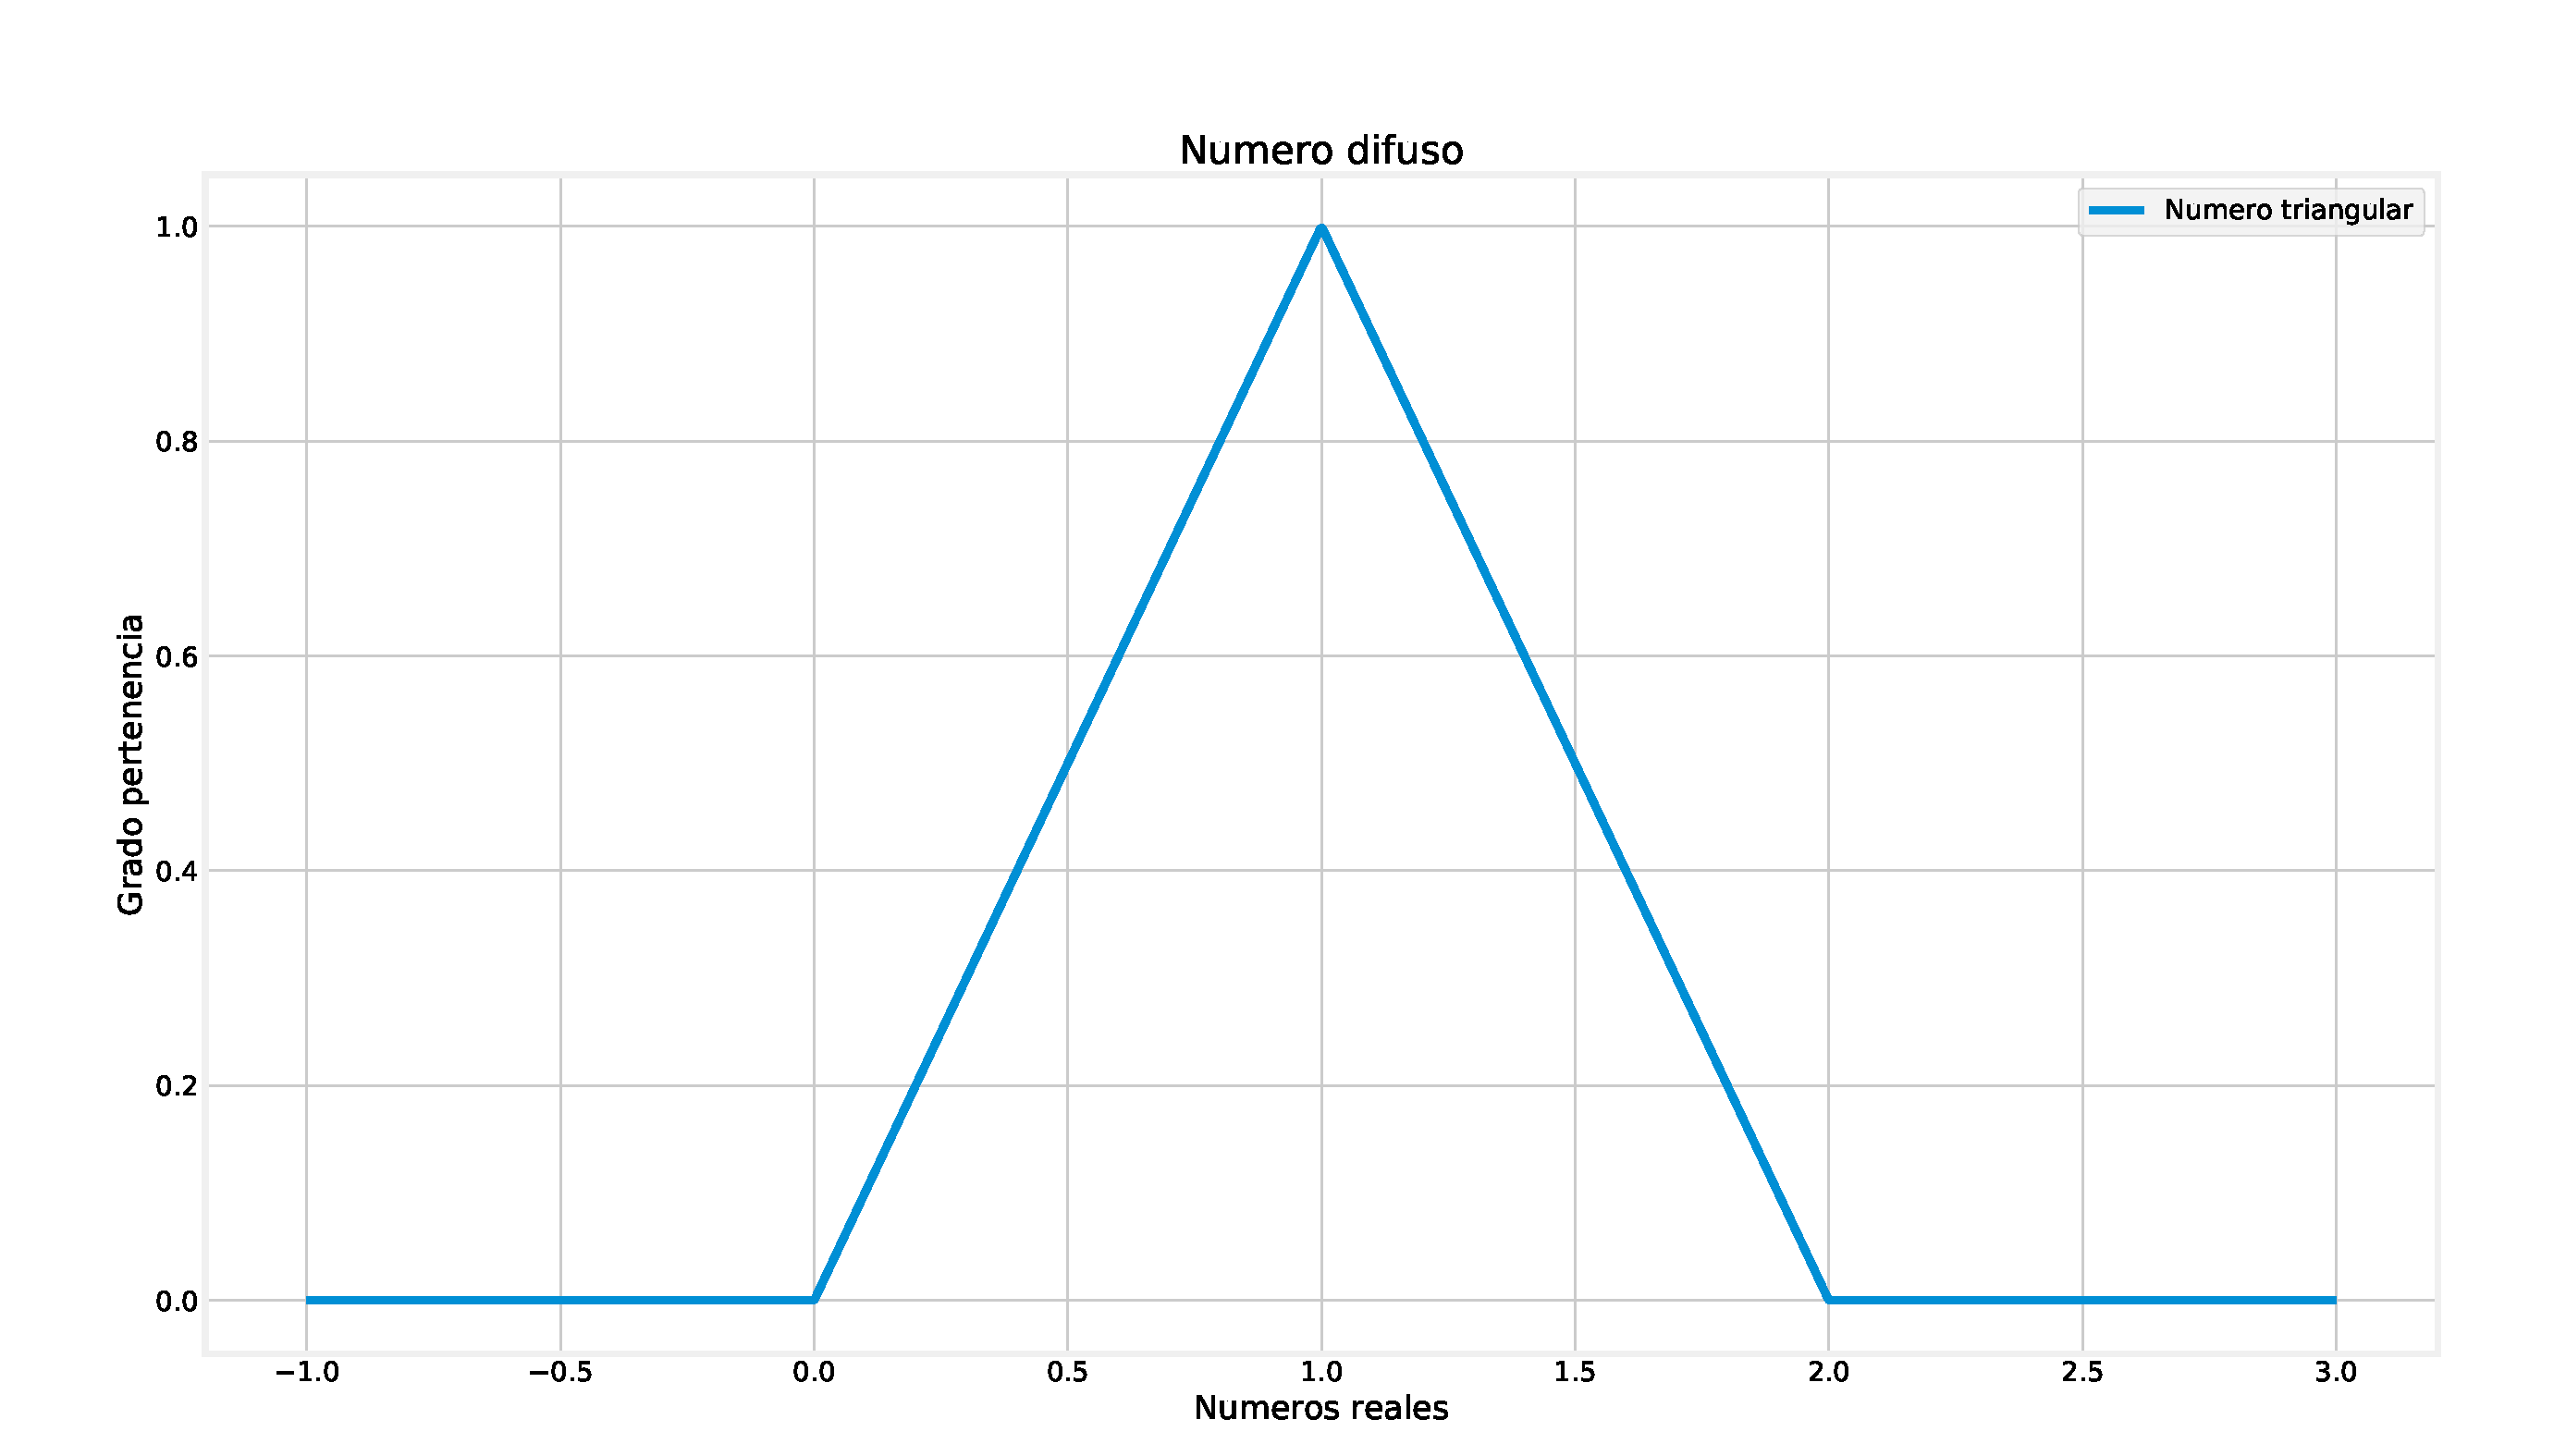
\includegraphics[width=\textwidth]{grafica_triangular}}
	\caption{Ejemplo de número triangular}
\end{figure}
Por otro lado, como ocurren en los números reales, también se le pueden asociar operaciones aritméticas básicas como la suma, el producto, la resta y la división. Las definiciones de suma, producto y división de números difusos funciona de forma bastante intuitiva, sin embargo, definir el concepto de resta de dos números difusos es más complejo, concepto que nos permitirá introducir derivadas de subconjuntos difusos, que es uno de los objetivos.
\\ \\
Otro concepto interesante a tener en cuenta y que marcó una revolución es la introducción del \hyperref[def:zadeh]{principio de extensión de Zadeh} \cite{fuzzyintro}, que permite calcular la imagen de un conjunto difuso mediante una función real. Todos estos conceptos introducidos por Lotfi A. Zadeh dan lugar a un marco teórico que permite desarrollar conceptos clásicos del análisis matemático en un contexto difuso.

\section{Objetivos de este trabajo}
Este trabajo trata de generalizar el concepto de ecuación diferencial a un marco difuso utilizando herramientas difusas y técnicas computacionales avanzadas, lo que se quiere conseguir con este trabajo es:
\begin{itemize}
	\item Conocer el concepto de número difuso.
	
	\item Introducir teoremas clásicos del análisis mediante la teoría de conjuntos difusos.
	
	\item Desarrollar el concepto de ecuación diferencial difusa.
	
	\item Hacer un análisis bibliográfico de los conceptos de análisis difuso.
	
	\item Comparar las soluciones de una ecuación diferencial difusa y una ecuación diferencial ordinaria.
	
	\item Introducir técnicas informáticas avanzadas para mejorar el rendimiento de los algoritmos numéricos desarrollados.
	
	\item Trabajar tecnologías pensando en el medioambiente. Un software que consume menos energía es mejor para el medioambiente.
\end{itemize}